\section{The signal detection problem}
\begin{marginfigure}
	\centering
	%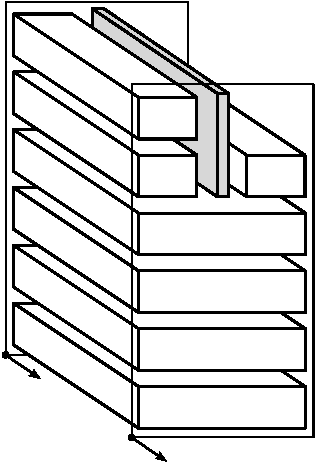
\includegraphics[scale=0.5]{ch3/img/PA_map_radar.pdf}
	\begin{tikzpicture}[>=latex',scale=0.4]
	\drawplanexy{-0.3}{-0.3}{-0.3}{6.7}{10}{dashed}{perception}
	
	\drawcube{0}{0}{5}{6.4}{1}{white}{dinamica}{}{};
	\drawcube{0}{1.2}{5}{6.4}{1}{white}{tracking}{}{};
	
	\drawcube{0}{2.4}{5}{6.4}{1}{white}{ostacoli}{}{};
	\drawcube{0}{3.6}{5}{6.4}{1}{white}{altitude}{}{};
	
	\drawcube{0}{4.8}{5}{3}{1.5}{white}{source}{}{};
	\drawcube{0}{6.5}{5}{3}{1.5}{white}{emulatore}{}{};

	\drawplanezy{3.2}{4.8}{5}{4.5}{radar_det}{fill=gray!40,opacity=0.90}{}{};

	\drawcube{3.4}{4.8}{5}{3}{3.2}{white}{alpha}{}{};
	\drawplanexy{-0.3}{-0.3}{5.3}{6.7}{10}{dashed}{action}
	

	\draw [->,line width=1.5] (action_D) -- ++(0,0,2);
	\draw [->,line width=1.5] (perception_D) -- ++(0,0,2);

	\coordinate [at=(radar_det_D), yshift=-5] (arrows_point);
	\draw [->,dashed]  (arrows_point) -- ++(1.5,0,0); 
	\draw [->,dashed]  (arrows_point) -- ++(-1.5,0,0); 
\end{tikzpicture}
\end{marginfigure}
We have two searching status for our agent. In one searching status, the VTOL tries to identify a signal presence, while in the second stage, once it has identified the presence of a signal, the drone has to find the transmission source point. The passage from a searching strategy to another is the \emph{supervised signal detection}.

\subsection{Supervised signal detection}
What we are trying to define is a strategy that is able to detect a target signal presence from a background noise. This is not new to signal theory, if we look at radar research work\citep{marcum1960statistical}.
\begin{marginfigure}
	\centering
	%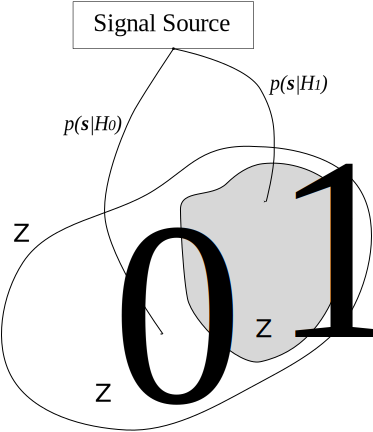
\includegraphics[scale=0.5]{ch3/img/signalsources.pdf}
	\begin{tikzpicture}[>=latex']
		\node [rectangle,inner sep=5pt,draw,xshift=-30] (src) {Signal Source};
		\draw [rotate=30](-2cm,-4cm) ellipse (2.5 and 1.5) node[xshift=45]{$\mathbb{Z}_0$};
		\draw [rotate=30,fill=gray!40](-2.5cm,-4cm) ellipse (1.2 and 0.75)node[xshift=15]{$\mathbb{Z}_1$};
		\node [yshift=-190] {$\mathbb{Z}$};
		\coordinate (z1) at (-0.75cm,-4.75cm);
		\coordinate (z0) at (1.7cm,-3.2cm);

		\draw [smooth,->] (src.east) .. controls (2cm,0cm) and (-2cm,-3cm) .. (z1) node[pos=0.5,left]{$p(\mathbf{s}|H_1)$};
		\draw [smooth,->] (src.east) .. controls (2cm,0cm) and (2cm, -1.5cm) .. (z0) node[pos=0.6,left]{$p(\mathbf{s}|H_0)$};
	\end{tikzpicture}
	\caption{Decision spaces}
\end{marginfigure}
The detection theory is seen as a binary classification problem based upon two hypothesis:
\begin{itemize}
\item hypothesis $0$: absence of signal
\item hypothesis $1$: presence of signal
\end{itemize}
The choice is made upon a signal ${\signal = [s_1,\dots,s_n]}$ in which a certain number of feature identifies its belonging to a decision field or observation space $\decspace \in \mathbb{R}^n$. The observation space is defined by the union of two decision regions:
\[ \decspace \equiv \decspacezero \cup \decspaceone \]
Each decision space has a conditional \emph{PDF}, that is assumed to be known:
\arraymath{
	\decspacezero & \mapsto & p(\signal|\hypzero) \\
	\decspaceone & \mapsto & p(\signal|\hypone) \\
}

\subsection{Risk criterion}
The classification is based upon criteria, such as:
\begin{itemize}
\item Minimum Risk Criterion
\item Minimax Criterion
\item Neyman--Pearson Criterion
\end{itemize}
That represents the classification strategies.

\myparagraph{Minimum risk criterion}
This criterion is based upon the assumptions that posteriors probability ${P(\hypzero|\signal)}$ and ${P(\hypone|\signal)}$ are known, and also the cost matrix is known, where the matrix is defined in table \ref{tbl:cost_matrix}.
\begin{margintable}
	\renewcommand{\arraystretch}{1}
	\begin{centering} 
		\begin{tabular}{>{\centering} m{1.25cm} <{\centering} | >{\centering} m{1.25cm} <{\centering} >{\centering} m{1.25cm} <{\centering}}
		\hline										& \scriptsize{\textbf{Decide absent}\newline$D_0$} & \scriptsize{\textbf{Decide present}\newline$D_1$} \tabularnewline \hline
		\scriptsize{\textbf{Signal absent}\newline$\hypzero$}  	& \cellcolor{lgray}\scriptsize{Correct rejection:\newline$c_{0,0}$} & \cellcolor{dgray}\scriptsize{False alarm:\newline$c_{1,0}$}        \tabularnewline
		\scriptsize{\textbf{Signal present}\newline$\hypone$} 	& \cellcolor{dgray}\scriptsize{Miss:\newline$c_{0,1}$}              & \cellcolor{lgray}\scriptsize{Hit:\newline$c_{1,1}$}                \tabularnewline \hline
		\end{tabular}
	\end{centering} 
	\renewcommand{\arraystretch}{1.75}
	\caption{Costs matrix}
	\label{tbl:cost_matrix}
\end{margintable}
In practice we have: ${c_{0,1} > c_{1,1}}$ and ${c_{1,0} > c_{0,0}}$.

The main objective is to \emph{minimize the average cost incurred by erroneous decision}\citep{duda2012pattern}. This is done through a minimization of a risk function defined over observation space. This optimization allows us to define the decision regions $\decspacezero$ and $\decspaceone$ which are optimal in terminal of overall risk. We define the risk:
\begin{equation}
R = c_{0,0} P(D_0, \hypzero) + c_{1,0} P(D_1, \hypzero) + c_{0,1} P(D_0, \hypone) + c_{1,1} P(D_1, \hypone)
\end{equation}
using the axiom of probability on $P(D_i,H_j)$, we get in general:
\begin{equation}
P(D_i,H_j) = P(D_i|H_j) P(H_j) \qquad (i,j) \in (0..1,0..1)
\end{equation}
and also:
\begin{equation}
P(D_i|H_j) = \int\limits_{\decspace_i}P(\signal|H_j)d\signal
\end{equation}
The evaluation, for each conditional probability is:
\begin{marginfigure} \label{fig:probdetection}
	\centering
	%\includegraphics[scale=0.55]{ch3/img/probcurves.pdf}
	\pgfmathdeclarefunction{gauss}{2}{%
		\pgfmathparse{1/(#2*sqrt(2*pi))*exp(-((x-#1)^2)/(2*#2^2))}%
	}
	\begin{tikzpicture}[>=latex']
		\begin{axis}[ 
			domain=0:12, samples=100,
		  	height=4cm, width=6cm,
			enlargelimits=false,
			axis lines=middle, 
			xlabel=\scriptsize{$\mathbf{s}$}, ylabel=\scriptsize{$p(\mathbf{s})$},
			every axis y label/.style={at=(current axis.above origin),anchor=south east},
		  	every axis x label/.style={at=(current axis.right of origin),anchor=west},
		  	xtick=\empty, ytick=\empty,
		  	extra x ticks={2.25,4.5,8.25},
		 	extra x tick labels={$\mathbb{Z}_0$,,$\mathbb{Z}_1$},
		  ]
		\addplot [fill=gray!40, draw=none, domain=0:4.5] {gauss(6.5,1.5)} \closedcycle;
		\addplot [fill=gray!75, draw=none, domain=4.5:12] {gauss(6.5,1.5)} \closedcycle;
		\addplot [black,line width=1.5] {gauss(4,1.3)};
		\addplot [black,line width=1.5] {gauss(6.5,1.5)};

		\end{axis}
		\node[xshift=85,yshift=70]{$p(\mathbf{s}|H_1)$};
		\node[xshift=27,yshift=77]{$p(\mathbf{s}|H_0)$};
		\draw  (1.665,0) -- ++(0,3.25) node[yshift=5]{$\leftarrow\mathbf{s}\rightarrow$};
		\draw (0.2,1)  -- node[above,pos=0.5]{$P_C$} ++(0.5,0) -- ++(-45:1.1);
		\draw (3,0.5) -- ++(45:1.1) -- ++(0.5,0) node[above,pos=0.5]{$P_D$};
		\end{tikzpicture} \\
		\begin{tikzpicture}[>=latex']
		\begin{axis}[ 
			domain=0:12, samples=100,
		  	height=4cm, width=6cm,
			enlargelimits=false,
			axis lines=middle, xlabel=\scriptsize{$\mathbf{s}$}, ylabel=\scriptsize{$p(\mathbf{s})$},
			every axis y label/.style={at=(current axis.above origin),anchor=south east},
		  	every axis x label/.style={at=(current axis.right of origin),anchor=west},
		  	xtick=\empty, ytick=\empty,
		  	extra x ticks={2.25,4.5,8.25},
		  	extra x tick labels={$\mathbb{Z}_0$,,$\mathbb{Z}_1$},
		  ]
		\addplot [fill=gray!40, draw=none, domain=4.5:12] {gauss(4,1.3)} \closedcycle;
		\addplot [fill=gray!75, draw=none, domain=0:4.5] {gauss(4,1.3)} \closedcycle;
		\addplot [black,line width=1.5] {gauss(4,1.3)};
		\addplot [black,line width=1.5] {gauss(6.5,1.5)};

		\end{axis}
		\node[xshift=85,yshift=70]{$p(\mathbf{s}|H_1)$};
		\node[xshift=27,yshift=77]{$p(\mathbf{s}|H_0)$};
		\draw  (1.665,0) -- ++(0,3.25) node[yshift=5]{$\leftarrow\mathbf{s}\rightarrow$};
		\draw (0.2,1)  -- node[above,pos=0.5]{$P_M$} ++(0.5,0) -- ++(-45:0.5);
		\draw (2,0.5) -- ++(25:1.5) -- ++(0.5,0) node[above,pos=0.5]{$P_F$};
		\end{tikzpicture}
	\caption{Probability versus decision space}
\end{marginfigure}
\arraymath{
	P(D_0|\hypzero) & = & \int\limits_{\decspacezero}p(\signal|\hypzero)d\signal = 1 - \probfalse \\
	P(D_0|\hypone) & = & \int\limits_{\decspacezero}p(\signal|\hypone)d\signal = \probmiss \\
	P(D_1|\hypzero) & = & \int\limits_{\decspaceone}p(\signal|\hypzero)d\signal = \probfalse \\
	P(D_1|\hypone) & = & \int\limits_{\decspaceone}p(\signal|\hypone)d\signal = 1 - \probmiss
}
where:
\begin{itemize}
\item $\probrej$: represents probability of correct rejection
\item $\probfalse$: represents probability of false alarm
\item $\probmiss$: represents probability of missed alarm
\item $\probdet$: represents probability of detection
\end{itemize}
and, looking at figure \ref{fig:probdetection}, stands the relation:
\arraymath{
	\probdet + \probmiss & = & 1 \\
	\probrej + \probfalse & = & 1
}

Finally, we get the defintion of risk:
\begin{equation}
\begin{array}{rcl} 
R & = & c_{0,0} \braces{1-\probfalse} P(\hypzero) + c_{0,1} \probmiss P(\hypone) + \\ 
  &   &  + c_{1,0} \probfalse P(\hypzero) + c_{1,1} (1-\probmiss) P(\hypone) \\
  & = & P(\hypzero) \braces{c_{0,0} + \probfalse (c_{1,0} - c_{0,0})} + P(\hypone) \braces{c_{1,1} + \probmiss (c_{0,1} - c_{1,1})}
\end{array}
\end{equation}
applying some substitutions:
\arraymath{
	\probmiss & = & \int\limits_{\decspacezero}p(\signal|\hypone)d\signal \\
	\probfalse & = & \int\limits_{\decspaceone}p(\signal|\hypzero)d\signal =  \\
	    & = & 1 - \int\limits_{\decspacezero}p(\signal|\hypzero)d\signal  \\
	1 & = & \int\limits_{\decspacezero}p(\signal|H_j)d\signal + \int\limits_{\decspaceone}p(\signal|H_j)d\signal 
}
and the risk equation:
\begin{equation}
\begin{array}{rcl}
R & = & P(\hypzero) \braces{c_{0,0} + \probfalse (c_{1,0} - c_{0,0})} + P(\hypone) \braces{c_{1,1} + \probmiss (c_{0,1} - c_{1,1})} = \\ 
  & = & P(\hypzero) \braces{c_{0,0} + \braces{1 - \int\limits_{\decspacezero}p(\signal|\hypzero)d\signal} (c_{1,0} - c_{0,0})} + \\ 
  &   &  + P(\hypone) \braces{c_{1,1} + \braces{\int\limits_{\decspacezero}p(\signal|\hypone)d\signal} (c_{0,1} - c_{1,1})} = \\ 
  & = & P(\hypzero) c_{1,0} + P(\hypone) c_{1,1} + \\
  &   & + \int\limits_{\decspacezero} P(\hypone)\braces{c_{0,1} - c_{1,1}} p(\signal|\hypone) - P(\hypzero)\braces{c_{1,0} - c_{0,0}} p(\signal|\hypzero) d\signal
\end{array}
\end{equation}
The first part is constant, to minimize the risk we have to work on the argument of the integral, that depends upon ${\decspacezero}$. Because:
\arraymath{
	P(\hypone)\braces{c_{0,1} - c_{1,1}} p(\signal|\hypone) & \geq & 0 \\
	P(\hypzero)\braces{c_{1,0} - c_{0,0}} p(\signal|\hypzero) & \geq & 0
}
the risk is minimized when:
\begin{equation}
P(\hypone)\braces{c_{0,1} - c_{1,1}} p(\signal|\hypone) < P(\hypzero)\braces{c_{1,0} - c_{0,0}} p(\signal|\hypzero)
\end{equation}
and rearranged as follow
\begin{equation}
\naming{ \dfrac{p(\signal|\hypone)}{p(\signal|\hypzero)} }{\likelihood} < \naming{ \dfrac{P(\hypzero)\braces{c_{1,0} - c_{0,0}}}{P(\hypone)\braces{c_{0,1} - c_{1,1}}} }{\threshold}
\end{equation}
that allow us to define the algorithm \ref{alg:minimumrisk}. Must be noticed:
\begin{itemize}
\item because of the binary nature, the decision rule obtained with the minimization on a single decision, grant the minimization of the risk also on the other decision; thus we could say that the local decision rule minimizes the overall risk
\item the likelihood ratio and threshold define decision regions as follows:
\arraymath{
	\decspacezero &=& \{ \signal\in\decspace \,:\,\likelihood<\threshold \} \\
	\decspaceone &=& \{ \signal\in\decspace \,:\,\likelihood>\threshold \} 
}
and a sample such that $\likelihood=\threshold$ could be assigned arbitrarily to one of the decision region
\item the distributions ${p(\signal|\hypzero)}$ and ${p(\signal|\hypone)}$ should be derived experimentally, something that is not to difficult because of characteristics of our signal
\end{itemize}
\begin{algorithm}[h]
\caption{Minimum risk criterion}
\label{alg:minimumrisk}
\KwData{ $p(\signal|\hypone),\,p(\signal|\hypzero),\,c_{0,0},\,c_{1,0},\,c_{0,1},\,c_{1,1}$ }
\tcc{Define the likelihood ratio}
$\likelihood \leftarrow \dfrac{p(\signal|\hypone)}{p(\signal|\hypzero)} $ \;
\tcc{Define the threshold}
$\threshold \leftarrow \dfrac{P(\hypzero)\braces{c_{1,0} - c_{0,0}}}{P(\hypone)\braces{c_{0,1} - c_{1,1}}}$ \;
\tcc{Binary classification}
\ForAll{$\signal_{in}$}{
	\eIf{$\Lambda(\signal_{in}) \leq \threshold$}{
		\Return{$\signal \in \hypzero$}
	}{
		\Return{$\signal \in \hypone$}
	}
}
\end{algorithm}

\myparagraph{The feature space}
The feature space that could be used are the three signal received from the three orthogonal antennas, plus the position. Te insertion of the position in the feature space is not important for the actual implementation, but could be useful in future, if some computer vision algorithm will be implemented. Algorithms that are able to represent symbolically the dimensions of the avalanche front, in conjunction with slope of the avalanche obtained by the altitude keeping routine, may allow us to define a probability distribution of the possible buried victims, distribution that could be inserted as a priori knowledge in radar detection and searching algorithm.
\FloatBarrier